%---------- Inleiding ---------------------------------------------------------

\section{Introductie} % The \section*{} command stops section numbering
\label{sec:introductie}

Zonder dat het te weten of te beseffen maakt de internetgebruiker continue gebruik van dataformaten en protocollen. Deze komen in verschillende soorten, XML, JSON, Protocol Buffers, GraphQL, ... Deze data formaten zorgen aan de hand van een achterliggende implementatie in een Application Programming Interface (API) voor dat mensen hun vrienden hun nieuwe Facebook of Instagrampost kunnen zien in een internetbrowser of op een app. 
APIs maken het meest gebruik van XML en JSON, indien toch een dominerend formaat gekozen moet worden zal dit JSON zijn. JSON is veel sneller om te lezen en te schrijven dan XML.

Echter wil dit niet zeggen dat JSON het snelste data formaat is. 
De Fashion Society is een moederbedrijf met verschillende kledingsketens onder zich. Om alles vlot te laten verlopen wordt gebruik gemaakt van een centraal beheersysteem voor zowat alles dat nodig is, dit houdt in maar is niet beperkt tot pickorders, webshops, ... Dit interne systeem maakt gebruik van het Façade patroon, dit is een structuur waar er maar één toegangspunt is tot een collectie ojecten met diensten en services. In het Façade patroon van de Fashion Society is de Orchestrator het toegangspunt tot een collectie van meerdere API’s, deze krijgt een request binnen voor een bepaalde service of dienst maar weet niet naar welke hij deze request moet doorsturen. Om dit op te lossen wordt gebruik gemaakt van de Discovery API, de Orchestrator zal deze aanroepen en de Discovery zal vervolgens de juiste Service ophalen en terugsturen naar de Orchestrator zodanig dat deze de originele request kan doorsturen naar de correcte API.

De Fashion Society wordt alsmaar groter en is op zoek naar een manier om de Discovery API performanter te laten wezen om zo meer realtime requests te kunnen afhandelen. De huidige Discovery API is een REST API dat gebruik maakt van JSON. In deze Bachelorproef zal onderzocht worden of Protocol Buffers ge¨ımplementeerd aan de hand van gRPC eventueel een even performant of zelfs performanter alternatief kan zijn voor de huidige implementatie van de Fashion Society dat gebruik maakt van een REST API met JSON. De bijhorende onderzoeksvragen zullen dan ook als volgt zijn:

\begin{itemize}
  \item Is gRPC met ProtocolBuffers sneller dan een REST API met JSON?
  \item Is gRPC met ProtocolBuffers efficiënter dan een REST API met JSON?
\end{itemize}

%---------- Stand van zaken ---------------------------------------------------

\section{State-of-the-art}
\label{sec:state-of-the-art}
gRPC is open source Remote Procedure Call (RPC) framework en is in 2015 ontstaan uit zijn voorganger Stubby, deze was een single general-purpose RPC infrastructuur~\autocite{gRPC}. Deze technologie laat het toe voor een programma om procedures te starten op andere computers in, eventueel, verschillende adresruimten aan de hand van een smal comminucatiekanaal~\autocite{Nelson1981}. gRPC zelf is geen dataformaat zoals JSON maar kan gebruik maken van verschillende data formaten, standaard is dit Protocol buffers, ook wel Protobufs genoemd.

JSON en Protocol Buffers hebben zowel gelijkenissen als grote verschillen, beide zijn een language-neutral dataformaat zo blijkt uit de documentatie van Protocol Buffers~\autocite{Google} en  JSON~\autocite{Json2017}. Het grootste, visuele verschil voor de gebruiker is te vinden in de structuur. JSON is een collectie van naam/value paren of een geordende lijst van waarden, daarintegen maken Protobufs gebruik van een soort model, er moet maar eenmaal gedefinieerd worden hoe de data gestructureerd zal zijn, daarna kan gebruik gemaakt worden van gegenereerde code om gemakkelijk data van en naar een variëteit van data streams te lezen en schrijven. Dit kan allemaal geprogrammeerd worden in heel wat verschillende programmeertalen.

gRPC wordt reeds gebruikt door verschillende grote bedrijven zoals Cisco en Netflix. 
Cisco gebruikt gRPC als het ideale, uniforme transportprotocol voor modelgestuurde configuratie en telemetrie. Dit komt dankzij de ondersteuning voor hoogwaardige bidirectionele streaming, op TLS gebaseerde beveiliging en het brede scala aan programmeertalen. 
Netflix koos dan weer voor gRPC omdat ze belang hechtte aan de architectonische kennis in de IDL (proto) dat een onderdeel is van gRPC en aan de, van deze proto-afgeleide, codegeneratie. Daarnaast speelde ook de cross-language compatibility en codegeneratie in gRPC een belangrijke rol bij de keuze voor gRPC bij Netflix~\autocite{Foundation2018}.

Eerder werd er nog geen officieel onderzoek uitgevoerd naar dit onderwerp, echter zijn wel online artikels te vinden die gRPC met REST gaan vergelijken aan de hand van een benchmark. Eén zo een onderzoek is uitgevoerd door~\textcite{Fernando2019}. Dit onderzoek was een benchmark tussen gRPC met Protocol Buffers en REST met JSON concludeerd dat gRPC sneller was dan REST behalve bij het streamen van data, hier is gRPC iets trager als REST.

Het onderzoek dat in deze Bachelorproef zal uitgevoerd worden is gebaseerd op dat van Ruwan Fernando, hiermee wordt bedoeld dat deze proof-of-concept geprogrammeerd zal worden in C\# en dat de  verschillende impelementaties met elkaar vergeleken zullen worden aan de hand van een benchmark. Het verschil met Fernando R. zijn onderzoek kan men vinden in de verwerking van de data, in dit onderzoek zal de data uit een aanhangende databank gehaald worden. Alsook zal in dit onderzoek een tienvoud van het aantal iteraties doen.

% Voor literatuurverwijzingen zijn er twee belangrijke commando's:
% \autocite{KEY} => (Auteur, jaartal) Gebruik dit als de naam van de auteur
%   geen onderdeel is van de zin.
% \textcite{KEY} => Auteur (jaartal)  Gebruik dit als de auteursnaam wel een
%   functie heeft in de zin (bv. ``Uit onderzoek door Doll & Hill (1954) bleek
%   ...'')

%---------- Methodologie ------------------------------------------------------
\section{Methodologie}
\label{sec:methodologie}
Het onderzoek zal gevoerd worden aan de hand van simulaties en experimenten in een Proof-of-Content (PoC). Er zullen 2 identieke APIs opgesteld worden in C\#, een .NET Core REST API voor JSON, en .NET Core API voor gRPC. Aan de hand van een benchmark tool, dewelke nog niet specifiek gekozen is, zullen er 2 verschillende categorieën aan GET en POST calls uitgevoerd worden. Big payload calls, hier zal substantief meer data opgehaald en verzonden worden dan bij de Small payload calls. Daarnaast zal het experiment meerdere malen uitgevoerd worden met 1000 en 2000 iteraties, dit om inaccurate metingen van kleine uitvoertijden te verminderen en een duidelijke conclusie te kunnen vormen.
Eens de resultaten van de experimenten verzameld zijn zullen we deze vergelijken en conclusies trekken.
%---------- Verwachte resultaten ----------------------------------------------
\section{Verwachte resultaten}
\label{sec:verwachte_resultaten}
Bij de grote payloads wordt een duidelijk verschil in voordeel van gRPC en Protocol Buffers verwacht, echter wordt er wel ook verwacht dat REST API met JSON in de kleine payloads nog degelijk zal presteren en misschien zelf nog licht overwegend beter zal zijn dan gRPC en Protocol Buffers.

%	\centering
%	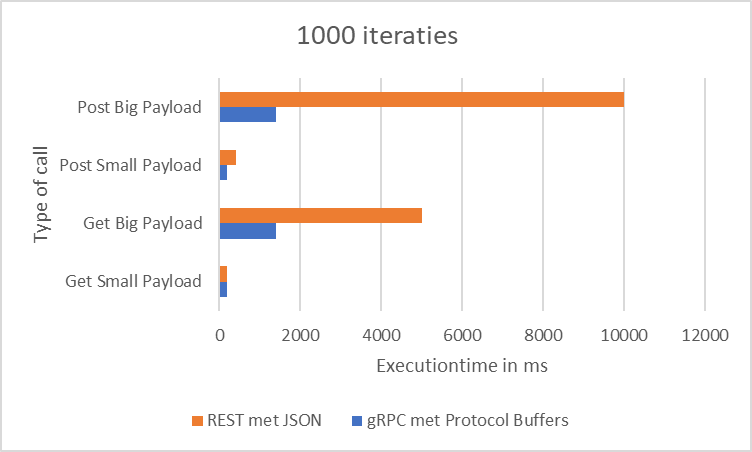
\includegraphics[width=1\linewidth]{screenshot001}



%	\centering
%	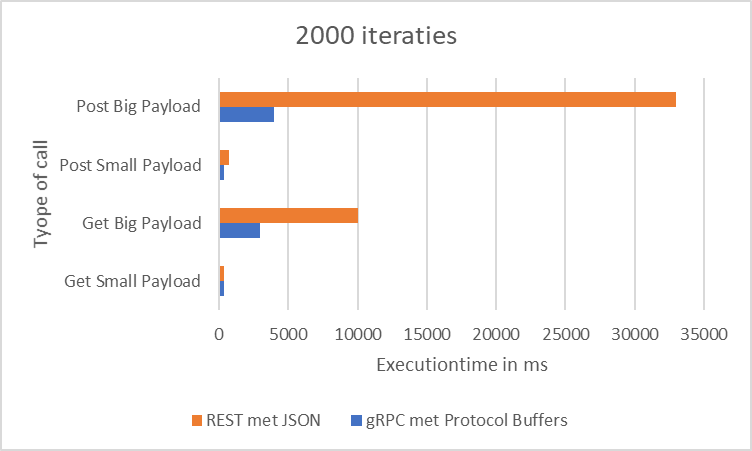
\includegraphics[width=1\linewidth]{screenshot002}

	



%---------- Verwachte conclusies ----------------------------------------------
\section{Verwachte conclusies}
\label{sec:verwachte_conclusies}

Dit onderzoek moet doen blijken of gRPC en Protocol Buffers sneller en efficiënter zijn dan een REST API met JSON. In de PoC zal duidelijk worden dat gRPC en Protocol Buffers een sneller en efficiënter alternatief zijn voor JSON. Dit resultaat zou eventueel verklaard kunnen worden doordat JSON een ouder dataformaat is en dus niet geoptimaliseerd is voor de huidige technologieën terwijl gRPC zeer recent ontworpen is om optimaal met de huidige technologieën om te gaan.

